%%%%%%%%%%%%%%%%%%%%%
% 3章
%%%%%%%%%%%%%%%%%%%%%
\chapter{ZDDを用いた区割列挙手法} \label{chapter:3}

\section{概要}

\section{ゼロサプレス型二分決定グラフ}
ゼロサプレス型二分決定グラフ(ZDD)は,組合せ集合を表す非巡回有向グラフで,
1993年に湊真一によって考案された\cite{minato}.
組合せ集合とは「$n$個のアイテムから任意個を選ぶ組合せ」を要素とする集合である.
$n$個のアイテムから任意個を選ぶ組合せは$2^n$通りあるので,
その組合せ集合は,$2^{2^n}$通り存在する.
例えば,$a,b,c$の3つの要素から組合せ集合を作る場合,
$\{ab, ac, c\}, \{a\}, \{\lambda, abc\}, \phi$などが挙げられる
($\lambda$は空の組合せ要素,$\phi$は空の集合を表す).

\begin{figure}[htbp]
  \begin{minipage}[b]{0.48\hsize}
    \centering
    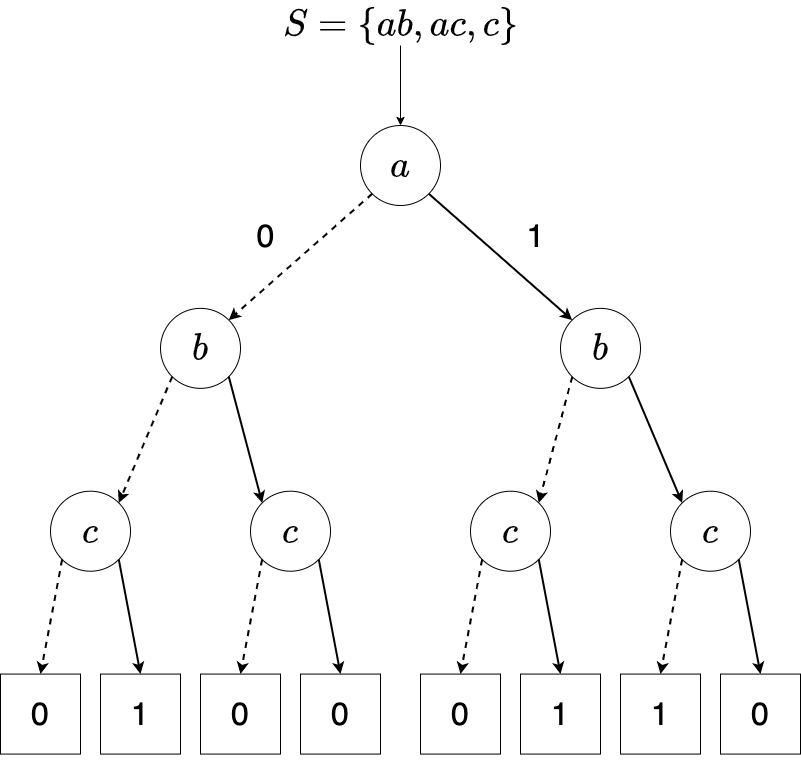
\includegraphics[scale=0.25]{img/binary_graph.png}
    \subcaption{場合分け二分木}
    \label{binary_graph}
  \end{minipage}
  \begin{minipage}[b]{0.48\hsize}
    \centering
    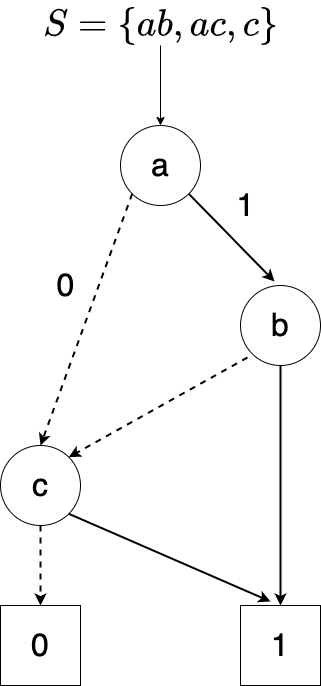
\includegraphics[scale=0.25]{img/zdd.png}
    \subcaption{ZDD}
    \label{zdd_graph}
  \end{minipage}
  \caption{組合せ集合$S=\{ab,ac,c\}$のグラフ表現}\label{combined_set}
\end{figure}

このような指数的な数の集合は,ZDDを用いることで効率的に表現することができる.
図\ref{combined_set}は,組合せ集合$S=\{ab,ac,c\}$を
場合分け二分木とZDDの両方で表した例である.
この二つのグラフは,各節点に要素を表すラベルが割り当てられていて,
0と1のラベルが付与された2種類の枝が分岐している.
そして葉には0または1の値が記入されている.
以降は0のラベルをもつ枝を0-枝(破線),1のラベルをもつ枝を1-枝(実線)とし,
また,0の値が記入された葉を0-終端(0-terminal),
1の値が記入された葉を1-終端(1-terminal)と呼ぶ.
これらのグラフでは,1-枝と0-枝はその接点の要素を選ぶかどうかの場合分けを表し,
葉の値はその葉に対応する組合せが集合に属するかを示している.

場合分け二分木とZDDを比較すると,ZDDは場合分け二分木で集合の表現に不要な頂点と枝を
削除していることがわかる.場合分け二分木から

ここで,ZDDの構造について述べる.
ZDDは有向非巡回グラフ$Z=(N,A)$によりデータ構造を表現する.
$N$は頂点集合,$A$は枝集合である.

\section{フロンティア法}

\section{区割列挙アルゴリズム}

\subsection{人口制約なしの場合}

\subsection{人口制約ありの場合}
